\documentclass{svproc}
\usepackage[T1]{fontenc}
\usepackage{graphicx,booktabs,amsmath,amssymb,array}
\usepackage{microtype}
\usepackage{xcolor,tikz,url}
\usetikzlibrary{arrows.meta,positioning,calc,fit,backgrounds}
\usepackage[hidelinks]{hyperref}
\hypersetup{pdftitle={Conservative Evidence Routing for Code Localization Agents},pdfsubject={CSRSE 2026 author-review draft},pdfkeywords={code localization, reliability, conservative pruning, evidence routing}}
\definecolor{navy}{HTML}{244A73}
\definecolor{teal}{HTML}{188477}
\definecolor{amber}{HTML}{D78A32}
\definecolor{ink}{HTML}{283849}
\definecolor{pale}{HTML}{EDF3F7}
\newcommand{\trace}{\textsc{Trace}}
\newcommand{\base}{CoSIL--Qwen3}
\newcommand{\hyb}{CoSIL--\trace}
\newcommand{\hit}{\operatorname{Hit}}
\newcommand{\rec}{\operatorname{Recall}}
\newcommand{\low}{\tau_{\mathrm{lo}}}
\newcommand{\high}{\tau_{\mathrm{hi}}}
\graphicspath{{figures/}}
\def\UrlFont{\rmfamily}
\setlength{\emergencystretch}{2em}

\begin{document}
\mainmatter
\title{Conservative Evidence Routing for Code Localization Agents}
\titlerunning{Conservative Evidence Routing for Code Localization}
\author{Author Names to Be Supplied}
\authorrunning{Author Names to Be Supplied}
\institute{Affiliation and corresponding-author details to be supplied}
\maketitle

\begin{abstract}
Code localization agents repeatedly decide which retrieved functions deserve further attention. These decisions offer an opportunity for smaller models, provided that evidence removal remains observable and uncertain cases receive further assessment. We present TRACE, a conservative routing layer combining function identity checks, calibrated relevance scoring, and escalation to the main agent. A structured evidence ledger connects retrieval, routing, source delivery, and final localization. In a paired study of 100 SWE-rebench tasks, a 4B reranker directly handles 323 of 652 scored requests and reduces main-model relevance-judgment tokens by 38.02\%. Both conditions achieve function Hit@5 of 49/92. No local rejection affects the 73 observed gold-function visits; these visits cover 57 of 117 gold identities. Total main-model tokens decrease by 4.65\%, while mean online latency increases by 14.85\%. The results characterize a measurable decision-substitution capability and establish an auditable basis for reliability-oriented agent integration.
\keywords{code localization, software reliability, selective prediction, evidence routing, language model agents}
\end{abstract}

\section{Introduction}
Repository-level issue localization narrows an issue report to files and functions for repair. Language-model agents combine repository search, code inspection, and iterative reasoning for this task~\cite{cosil2025,swebench2024}. Their effectiveness depends on the evidence reaching the model. A function can be present in the repository yet absent from the reasoning context because its file was overlooked, its identity was unresolved, or a relevance decision discarded its source.

Relevance judgments offer an integration point for smaller models: clear cases can be decided locally and uncertain ones sent to the main agent. This introduces a reliability question: \emph{which evidence was exposed to the smaller model, and what happened to it afterwards?} Answering it requires connecting local judgments to the evidence available throughout an agent trajectory.

We address this question through \trace{} (Traceable Relevance Assessment with Conservative Escalation), a function-level evidence-routing layer integrated into CoSIL. The layer binds retrieved code to repository identities, scores issue--function relevance with a trained Qwen3-Reranker-4B, and applies a conservative retain/reject/escalate policy. An event ledger links these decisions to source delivery and final predictions. The design gives an explicit operational role to uncertainty: intermediate scores preserve access to the original Qwen3-8B judgment pathway.

The study makes three contributions. First, it describes a reproducible integration of function-aware scoring and conservative escalation within an iterative localization agent, including identity checks and a shared input renderer. Second, it introduces an evidence-chain assessment that reports local target rejection together with target exposure, source delivery, and endpoint localization. Third, it provides a paired 100-repository study and offline threshold replay, quantifying decision substitution, resource use, and where localization opportunities are lost. Together these contributions turn a relevance classifier into an inspectable component of an agent system.

We investigate three questions: how much judgment work can be delegated while preserving observed target evidence; how this changes localization and resource use; and where evidence is lost along the workflow. The smaller model handles 49.54\% of scored decisions directly, judgment tokens fall by 38.02\%, and aggregate function Hit@5 remains 49/92 in the observed run.

\section{Background and Design Rationale}
CoSIL moves from file localization to function candidates through iterative code-graph search, relevance assessment, and reflection~\cite{cosil2025}. Source admission is a distinct decision point: our baseline uses the main model, while the proposed condition delegates clear function judgments to a smaller scorer.

Qwen3 Reranker models express relevance through \texttt{yes}/\texttt{no} likelihoods~\cite{qwen3embedding2025}, enabling score extraction without rationale generation. We use an existing frozen LoRA adapter, a parameter-efficient adaptation method~\cite{hu2021lora}.

Temperature scaling calibrates score magnitudes~\cite{guo2017calibration}, while selective prediction formalizes the option to defer uncertain decisions~\cite{geifman2019selectivenet}. LLM cascades and routers likewise explore allocating requests across models~\cite{frugalgpt2023,routellm2024}. \trace{} applies these established ingredients at the \emph{retrieved-code evidence boundary}. Its distinctive emphasis is the link between an individual routing decision and the evidence available to later agent steps. The evaluation therefore includes exposure and delivery measures alongside conventional ranking metrics.

SWE-bench and SWE-rebench provide repository issues and reference repairs~\cite{swebench2024,swerebench2025}. Our isolated evaluator uses reference changes to identify existing target functions; both agents inspect only the issue's base revision.

\section{Method}
\subsection{Function-Aware Evidence Interface}
Figure~\ref{fig:architecture} shows the integration. A localization step requests a file, class, or function from the base-revision repository inventory. For a function request, the integration resolves a canonical identity consisting of its relative file path and qualified function name. The source range and identity header are checked against that inventory before a scoring request is constructed. Generic feedback helps the agent correct an unavailable path or an incorrect owner, such as a module-level function requested as a class method. Both experimental conditions use these same engineering checks.

\begin{figure}[t]
\centering
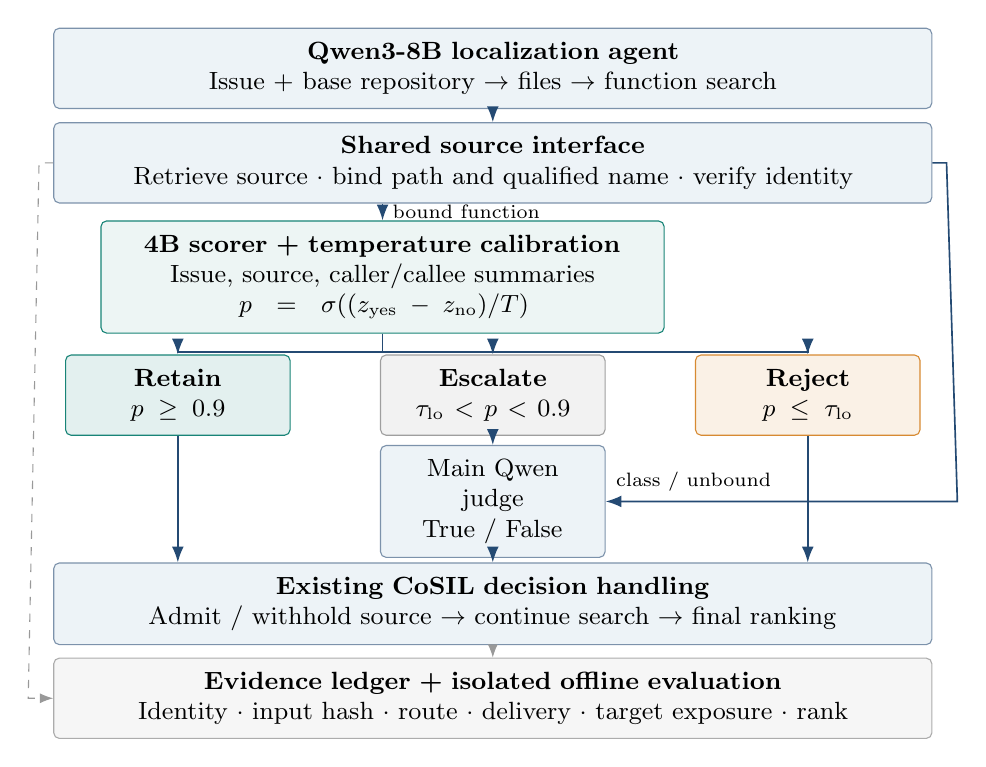
\begin{tikzpicture}[
  font=\small, >=Latex,
  box/.style={draw=navy!60,rounded corners=2pt,fill=pale,align=center,inner sep=5pt,minimum height=0.8cm},
  route/.style={box,text width=2.5cm,minimum height=0.85cm},
  link/.style={->,semithick,draw=navy},
  audit/.style={->,dashed,draw=gray!80,thin}]
  \node[box,text width=10.8cm] (agent) at (0,0) {\textbf{Qwen3-8B localization agent}\\Issue + base repository $\rightarrow$ files $\rightarrow$ function search};
  \node[box,text width=10.8cm] (identity) at (0,-1.2) {\textbf{Shared source interface}\\Retrieve source $\cdot$ bind path and qualified name $\cdot$ verify identity};
  \draw[link] (agent)--(identity);
  \node[box,fill=teal!8,draw=teal,text width=6.8cm] (score) at (-1.4,-2.65) {\textbf{4B scorer + temperature calibration}\\Issue, source, caller/callee summaries\\$p=\sigma((z_{\mathrm{yes}}-z_{\mathrm{no}})/T)$};
  \draw[link] (identity.south -| score.north)--node[right,font=\scriptsize]{bound function}(score.north);
  \node[route,fill=teal!12,draw=teal] (keep) at (-4,-4.15) {\textbf{Retain}\\$p\geq0.9$};
  \node[route,fill=gray!10,draw=gray!75] (defer) at (0,-4.15) {\textbf{Escalate}\\$\tau_{\mathrm{lo}}<p<0.9$};
  \node[route,fill=amber!12,draw=amber] (drop) at (4,-4.15) {\textbf{Reject}\\$p\leq\tau_{\mathrm{lo}}$};
  \draw[link] (score.south)--++(0,-.23)-|(keep.north);
  \draw[link] (score.south)--++(0,-.23)-|(defer.north);
  \draw[link] (score.south)--++(0,-.23)-|(drop.north);
  \node[box,text width=2.5cm] (qwen) at (0,-5.5) {Main Qwen judge\\True / False};
  \draw[link] (defer)--(qwen);
  \draw[link] (identity.east)--++(.18,0)--(5.9,-5.5)--node[above,font=\scriptsize,near end]{class / unbound}(qwen.east);
  \node[box,text width=10.8cm] (delivery) at (0,-6.8) {\textbf{Existing CoSIL decision handling}\\Admit / withhold source $\rightarrow$ continue search $\rightarrow$ final ranking};
  \draw[link] (keep.south)--(keep.south|-delivery.north);
  \draw[link] (drop.south)--(drop.south|-delivery.north);
  \draw[link] (qwen)--(delivery);
  \node[box,text width=10.8cm,fill=gray!7,draw=gray!65] (ledger) at (0,-8) {\textbf{Evidence ledger + isolated offline evaluation}\\Identity $\cdot$ input hash $\cdot$ route $\cdot$ delivery $\cdot$ target exposure $\cdot$ rank};
  \draw[audit] (delivery)--(ledger);
  \draw[audit] (identity.west)--++(-.18,0)--(-5.9,-8)--(ledger.west);
\end{tikzpicture}

\caption{\trace{} at the source-admission boundary. The main agent retains control of search and ranking. Dashed links record evidence; reference targets are joined only by the offline evaluator. The baseline uses the same tool and identity interface, with every relevance judgment routed to Qwen3-8B.}
\label{fig:architecture}
\end{figure}

Each scoring request is bound to a canonical function identity. Model input contains the issue, function source, and summaries of direct callers and callees from the base-revision structure. The shared renderer caps issue text at 8,000 characters and function text at 8,192 characters, with 16 neighbors per direction. Packing enforces an 8,128-token prompt ceiling, removing neighbors before shortening text. Input hashes record the exact scored representation.

Class requests and unresolved bindings follow the main-model pathway. The final ranking is evaluated as emitted, without gold-based identity corrections.

\subsection{Calibrated Three-Way Routing}
Let $x$ denote the rendered issue--function input. The adapted reranker produces the logits $z_{\mathrm{yes}}(x)$ and $z_{\mathrm{no}}(x)$ at the final prompt position. Its calibrated relevance score is
\begin{equation}
 p(x)=\sigma\!\left(\frac{z_{\mathrm{yes}}(x)-z_{\mathrm{no}}(x)}{T}\right),
 \qquad \sigma(u)=\frac{1}{1+e^{-u}}.
 \label{eq:score}
\end{equation}
The temperature $T$ is fitted on the existing validation split. The routing policy is
\begin{equation}
 r(x)=\begin{cases}
 \textsc{Reject}, & p(x)\leq\low,\\
 \textsc{Retain}, & p(x)\geq\high,\\
 \textsc{Escalate}, & \low<p(x)<\high.
 \end{cases}
 \label{eq:route}
\end{equation}
Retention and rejection substitute for the original relevance decision; escalation asks the main Qwen3-8B judge. Rejected source is withheld, and the agent is prompted to select another node rather than explore its callees. Search continues, with up to ten function-tool selections. The scorer generates no explanation tokens. Scores, decisions, identities, and input hashes are logged together.

We deploy $T=2.9846201$ and $\high=0.9$. The lower threshold, $\low\approx0.129476$, is the largest representable value strictly below the minimum calibrated validation gold-function score:
\begin{equation}
 \low=\operatorname{nextafter}\!\left(\min_{x\in G_{\mathrm{val}}}p(x),-\infty\right).
 \label{eq:threshold}
\end{equation}
Direct rejection therefore starts below every observed validation target score. The upper threshold retains high-confidence functions, and intermediate scores receive main-model assessment. All values are frozen before the study.

The existing adapter uses 8,556 training pairs from 359 issues and 487 validation pairs from 44 different issues, drawn from issue-disjoint subsets of SWE-bench Lite and additional Verified tasks. Positives combine modified functions and direct-call proxies; negatives follow frozen static and runtime qualification rules. Weighted yes/no cross-entropy preserves a 1:2 positive-to-negative total weight. LoRA uses rank 16, scaling 32, dropout 0.05, learning rate $5\!\times\!10^{-5}$, and effective batch size 8. We retain epoch 1 from the preceding diagnostic training study (validation accuracy 88.09\%, AUROC 0.9470), without adaptation on Rebench.

\subsection{Evidence-Chain Reliability Assessment}
The ledger links file selection, source retrieval, routing, source delivery, and ranking. Each record is associated with its task, base revision, canonical object identity, and step/event; input hashes and source references connect scoring and delivery. A tool returning source and the search agent receiving it are separate events. Reference targets are joined only during offline evaluation.

Three measures describe local routing. \emph{Automatic decision coverage} is the fraction of scored requests directly retained or rejected. \emph{Observed target rejection} is the fraction of scored gold-function visits directly rejected. \emph{Target exposure} is the fraction of unique reference function identities that actually receive a local score. Reporting all three clarifies both the amount of judgment substitution and the portion of the task to which the observed safety evidence applies. Repeated visits are counted as events for routing, but deduplicated for identity exposure.

For unsuccessful tasks, the ledger identifies the observable gap: target file absent, selected file without target retrieval, delivered source without a top-five target, or resource failure. This decomposition assigns follow-up engineering to a specific workflow stage.

\section{Experimental Design}
\subsection{Frozen Tasks and Paired Conditions}
We use the frozen SWE-rebench leaderboard snapshot (revision \texttt{34d5a588}, full identifier in the artifact manifest). Its existing 265-task pool applies four Lite-style conditions: the business repair patch changes at most one file and three diff hunks, creates/deletes no files, and the issue has at least 40 words. Previously recorded repository exclusions are retained.

Sampling uses seed 20261110 and SHA256 of the UTF-8 seed, a colon, and the task identifier. We sort by hash then identifier, keep one task per case-folded repository, and select the first 100. Neither predictions nor function evaluability enter selection. This gives a prespecified development diagnosis of 100 tasks from 100 repositories.

Table~\ref{tab:configuration} summarizes the paired design. Both conditions use Qwen3-8B in non-thinking mode. The baseline uses the original main-model relevance judgment; \trace{} substitutes the three-way local route. Each baseline file-selection phase is newly executed and shared with its paired \trace{} run. Subsequent function planning, exploration, and ranking execute independently. Thus the comparison concentrates on integration within function search while holding the file-stage result fixed.

\begin{table}[t]
\caption{Frozen paired configuration. The artifact manifest contains full model revisions and adapter hashes.}
\label{tab:configuration}
\centering\small
\begin{tabular}{@{}p{0.29\textwidth}p{0.66\textwidth}@{}}
\toprule
Component & Setting \\
\midrule
Main agent, both arms & Qwen3-8B; BF16; non-thinking; temperature 0; seed 0; 65,536 context / 2,048 output tokens \\
Baseline relevance & Qwen3-8B True/False judgment \\
\trace{} relevance & Frozen Qwen3-Reranker-4B LoRA; Eq.~\ref{eq:route}; class/unbound requests use Qwen3 \\
Shared controls & Base revision, file stage, tool identity checks, source interface, scoring convention \\
Local inputs & Issue 8,000 chars; function 8,192 chars; 16 neighbors/direction; 8,128-token packed ceiling \\
Hardware & Two RTX 3090 GPUs; tensor-parallel main model; resident scorer shares the second GPU \\
Evaluation set & 100 fixed tasks; 92 with complete nonempty existing-function targets \\
\bottomrule
\end{tabular}
\end{table}

Ninety-nine tasks complete both conditions. One repository directory exceeds the context limit before the first request; its resource failure and paired shared-stage blockage remain in the fixed set. The controller resumes only unexecuted tasks, preserving prior records.

\subsection{Metrics and Accounting}
The R2 evaluator maps reference changes through exact patch-context offsets and AST ranges. Function metrics include the 92 tasks with complete, nonempty existing-function targets; the other eight are function-level NA. File metrics use all 100 tasks. Failures retain their applicable denominators.

For task $i$, let $G_i$ be the existing target-function set and $P_i^k$ the distinct valid identities present within the first $k$ emitted rank slots. Strict relative-path and qualified-name equality determines matches. Invalid, repeated, or class-only slots are not compressed. We report
\begin{align}
 \hit_i@k&=\mathbf{1}[P_i^k\cap G_i\ne\varnothing], &
 \rec_i@5&=\frac{|P_i^5\cap G_i|}{|G_i|},\\
 \operatorname{Prec}_i@5&=\frac{|P_i^5\cap G_i|}{5}, &
 \operatorname{All}_i@5&=\mathbf{1}[G_i\subseteq P_i^5].
\end{align}
Macro precision, recall, and F1 average the per-task values. Hit confidence intervals use Wilson's method. The paired Hit@5 difference uses 5,000 task-bootstrap draws with seed 20261110, accompanied by an exact McNemar test.

Comparable resource totals charge shared file-stage tokens and time to both arms; the actual batch ledger counts them once. Main-model and scorer tokens remain separate. Online latency includes rendering, calls, and scoring for the same 99 completed pairs; preparation and startup are reported separately.

\subsection{Offline Threshold Replay}
We replay lower thresholds on frozen scores with $\high=0.9$, measuring automatic coverage and target-visit rejection on 487 validation pairs and 652 runtime requests. This requires no additional model calls and provides a score-level sensitivity analysis.

\section{Results}
\subsection{Local Decision Substitution and Target Exposure}
Of 652 scored requests, \trace{} directly retains 219, rejects 104, and escalates 329. Thus 323/652 requests (49.54\%) receive a local decision. Twelve binding/rendering fallbacks follow the main-model route outside this scored-request denominator; class requests also remain with the main model. The scorer's median decision latency is 0.185 seconds, with a 95th percentile of 0.513 seconds.

\begin{figure}[t]
\centering
\includegraphics[width=\textwidth]{fig_routing.pdf}
\caption{Decision substitution and target exposure. Routing counts use scored requests; exposure uses unique gold identities; gold routes use observed visits. These separate denominators make the scope of each measurement explicit.}
\label{fig:routing}
\end{figure}

The local scorer encounters 57 of the 117 unique existing target identities, represented by 73 visits. It directly retains 60 visits and escalates 13, with zero direct target rejections (Fig.~\ref{fig:routing}). This is the observed evidence-preservation behavior at the local decision boundary. It is particularly useful alongside automatic coverage: nearly half the scored requests are handled locally while every observed target visit is either retained or receives the original model's assessment.

Figure~\ref{fig:thresholds} makes the operating trade-off explicit. At a lower threshold of 0.6, replay rejects 11/76 validation target examples and 4/73 runtime target visits. Compared with 0.6, the deployed threshold transfers 125 of the recorded runtime decisions from rejection to escalation, including those four target visits. Automatic coverage changes from 68.71\% to 49.54\%. This quantifies the additional assessment allocated to uncertain evidence on the frozen traces.

\begin{figure}[t]
\centering
\includegraphics[width=\textwidth]{fig_threshold_replay.pdf}
\caption{Offline lower-threshold replay with the retain threshold fixed at 0.9. The validation and observed runtime populations are distinct. The deployed point is frozen before the runtime study; these curves describe recorded scores, not new end-to-end runs.}
\label{fig:thresholds}
\end{figure}

\subsection{Localization Outcomes}
Table~\ref{tab:outcomes} reports the endpoint results. File Hit@5 is 68/100 in both conditions because the file phase is shared. Function Hit@5 is 49/92 (53.26\%) in both, with a Wilson 95\% interval of 43.14--63.12\%. \trace{} has one additional Hit@1 and Hit@3; full-target coverage is 39/92 compared with 40/92 for the baseline. The paired Hit@5 table contains 48 joint hits, one baseline-only hit, one \trace{}-only hit, and 42 joint misses. The difference is 0.00 percentage points, with paired 95\% interval $[-3.26,3.26]$ and exact McNemar $p=1.0$.

\begin{table}[t]
\caption{Localization outcomes on the fixed sample. Function proportions use the 92 eligible tasks; macro metrics are averages over the same 92 tasks.}
\label{tab:outcomes}
\centering\small
\begin{tabular}{@{}lrr@{}}
\toprule
Metric & \base{} & \hyb{} \\
\midrule
File Hit@1 & 48/100 (48.00\%) & 48/100 (48.00\%) \\
File Hit@3 & 59/100 (59.00\%) & 59/100 (59.00\%) \\
File Hit@5 & 68/100 (68.00\%) & 68/100 (68.00\%) \\
\midrule
Function Hit@1 & 36/92 (39.13\%) & 37/92 (40.22\%) \\
Function Hit@3 & 47/92 (51.09\%) & 48/92 (52.17\%) \\
\textbf{Function Hit@5} & \textbf{49/92 (53.26\%)} & \textbf{49/92 (53.26\%)} \\
Macro Precision@5 & 11.74\% & 11.52\% \\
Macro Recall@5 & 48.10\% & 47.55\% \\
Macro F1@5 & 18.51\% & 18.20\% \\
All existing targets@5 & 40/92 (43.48\%) & 39/92 (42.39\%) \\
Function MRR@10 & 0.4518 & 0.4592 \\
\bottomrule
\end{tabular}
\end{table}

The smaller model substitutes for a substantial share of judgments while the observed aggregate top-five endpoint is maintained. Recall and all-target coverage additionally distinguish finding one target from covering all targets.

\subsection{Token Use and Online Latency}
Main-model judgment tokens decrease by 38.02\% (Table~\ref{tab:resources}). Full-pipeline main-model tokens decrease by 386,154 (4.65\%). The 4B scorer consumes 764,211 input tokens and generates no output tokens. Actual batch main-model usage is 15,623,261 tokens, with the shared file phase counted once.

\begin{table}[t]
\caption{Resource accounting. Comparable totals include the same file-phase charge (617,293 tokens) for each arm. Online statistics use 99 completed pairs.}
\label{tab:resources}
\centering\small
\begin{tabular}{@{}l@{\hspace{7pt}}r@{\hspace{11pt}}r@{}}
\toprule
Quantity & \base{} & \hyb{} \\
\midrule
Comparable main-model tokens & 8,313,354 & 7,927,200 \\
Main relevance-judgment tokens & 964,727 & 597,941 \\
Additional 4B input tokens & --- & 764,211 \\
Mean main tokens per completed task & 83,973.27 & 80,072.73 \\
Mean online time (s/task) & 34.89 & 40.07 \\
Median online time (s/task) & 33.77 & 38.87 \\
Paid API expenditure & \$0 & \$0 \\
\bottomrule
\end{tabular}
\end{table}

Mean online time increases from 34.89 to 40.07 seconds (14.85\%). Local scoring precedes escalation, with the scorer sharing a GPU with the main model. CPU cache preparation takes 255.47 seconds; scorer loading takes 4.80 and 7.82 seconds in the two service sessions, excluding imports and main-model startup.

The resulting resource profile is useful for deployment planning: judgment-token reduction and wall-clock improvement are separate objectives. The current configuration provides measured main-model substitution, with latency identifying batching and scheduling as concrete optimization targets.

\subsection{Evidence-Chain Findings}
Figure~\ref{fig:outcomes} connects endpoint accuracy to the stage of the observable miss. Each arm has 43 function Hit@5 misses. In 30 of these, the target file is absent from the selected set and target source is never retrieved. Another nine baseline and eleven \trace{} misses select a target file without retrieving its target function. Target source is delivered but absent from the final top five in three baseline and one \trace{} cases. The remaining case is the shared context-limit failure.

\begin{figure}[t]
\centering
\includegraphics[width=\textwidth]{fig_outcomes.pdf}
\caption{Endpoint localization and observable gaps. The left panel uses 92 function-evaluable tasks per arm; the right partitions the 43 misses per arm. The audit identifies which stage lacks the target evidence, supporting focused follow-up engineering.}
\label{fig:outcomes}
\end{figure}

The decomposition identifies where the component can act: scoring begins only after retrieval. The trace accordingly separates local evidence preservation from opportunities to improve file selection and function exploration.

In the Strands SDK, both judges reject the target \nolinkurl{LiteLLMModel.structured_output}. Its score of 0.3918 follows the configured escalation route. Both arms achieve Hit@5 through another target, but Recall@5 is 0.5. The ledger exposes this partial evidence loss behind a successful hit.

For the two discordant Hit@5 tasks, the first function-planning requests are identical between arms but their responses already differ before any local scoring. In the baseline-only case, all ten scored requests take the escalation route and the missed target is never retrieved. In the \trace{}-only case, both arms retrieve and admit the target source, but the final ranking differs. The trace therefore distinguishes a routing event from other trajectory changes instead of treating every paired win or loss as a direct consequence of pruning.

\section{Reliability Implications and Limitations}
\subsection{An Operational Contract for Evidence Routing}
Three elements make the integration useful for reliability-oriented evaluation. \emph{Identity continuity} connects a model-requested object to the source that is actually scored and delivered. \emph{Conservative escalation} gives ambiguous scores an explicit continuation path through the original judge. \emph{Exposure-aware auditing} states both how much local work is substituted and which target identities are covered by the observation. These elements provide a practical contract for assessing a learned component inside an agent.

The engineering history further motivates this contract. In the preceding 17 function-evaluable development tasks, shared identity and path repairs increased hits from 10 to 12 in both arms. That result belongs to the tool interface rather than the smaller scorer. Accordingly, the present paired study gives both conditions the repaired interface. This keeps common engineering improvements separate from the contribution of judgment substitution.

The evidence ledger is also a reusable diagnostic artifact. It distinguishes source extraction from source delivery, captures resource failures before model invocation, and relates local decisions to task outcomes. Independent validation checks 3,440 main-model requests, 1,409 source-return records, 4,961 delivery events, and 652 scored routes; 39 CPU tests exercise the integration and continuation controls. This level of traceability enables reproducible inspection of where evidence enters or leaves the workflow.

\subsection{Scope and Threats to Validity}
The 100-task pool is a development sample with prior experimental observation, one task per repository, and four explicit patch/issue filters. It does not represent all SWE-rebench tasks. Training labels include static-call proxies and qualified negatives, so validation accuracy describes those labels rather than complete semantic relevance. Unmodified helper functions can still be important; the 104 rejected non-gold requests therefore cannot be interpreted as 104 proven correct exclusions.

Temperature and the lower threshold use the same validation split. Zero validation target rejection follows by construction and does not certify future risk. Runtime zero rejection is conditional on 73 observed target visits covering 57 identities; unseen targets remain outside that observation. Earlier validation risk gates did not certify the checkpoint, and this deployment is a diagnostic evaluation of a subsequently conservative operating point.

The experiment has one generation per condition. Across the 99 completed pairs, identical first function-planning requests produce different replies in 83 cases even with temperature and seed set to zero. Shared file selection controls one source of variation, while subsequent trajectories can diverge. The paired interval and McNemar result do not establish equivalence or non-inferiority, and individual changes cannot be uniquely attributed to local routing. The scorer and main agent also belong to the same model family.

The 4B input renderer may shorten source to satisfy its frozen token limit. Reference targets follow the evaluator's existing-function definition and AST mapping, not every possible valid repair strategy. No repair tests are performed. Latency is affected by the fixed baseline-first order, caching, and shared GPU placement; reduced main-model tokens do not directly measure total energy or hardware cost. Offline threshold replay keeps observed visits fixed and cannot predict the online accuracy of a changed policy.

\section{Conclusion}
\trace{} combines function-aware scoring, conservative escalation, and an evidence ledger to make local relevance decisions inspectable within a code localization agent. In the paired study, it directly handles 49.54\% of scored requests, reduces main-model judgment tokens by 38.02\%, and retains an observed aggregate function Hit@5 of 49/92. Its exposure-aware audit records zero direct rejection across 73 observed target visits and identifies upstream search as the dominant location of missing target evidence. The contribution is an operationally explicit approach to integrating and assessing a smaller model at the code-evidence boundary. Future work can use the same trace contract to evaluate improved candidate retrieval and more efficient scoring schedules.

\paragraph{Artifacts and disclosure.}
Code, derived data, figures, and configuration identifiers accompany this draft\footnote{\url{https://github.com/dantongwangwww/cosil_repro}, under \texttt{CoSIL/papers/csrse2026\_pruning}.}. AI assistance supported code, analysis, visualization, and drafting. Author verification and final disclosure are pending in this review draft.

\bibliographystyle{spmpsci}
\bibliography{references}
\end{document}
